\documentclass[a4paper,10pt]{article}

\usepackage[utf8]{inputenc}
\usepackage[francais]{babel}
\usepackage[T1]{fontenc}
\usepackage{graphicx}
\usepackage{epsfig}
\usepackage[top=2cm, bottom=2cm, left=2cm, right=2cm]{geometry}
\usepackage[protrusion=true,expansion=true]{microtype}	
\usepackage{amsmath,amsfonts,amsthm,amssymb}
\usepackage{listings}
\lstset{
basicstyle=\small,
language=Prolog,
frame=single,
}


\usepackage[dvips]{hyperref}

%\title{Rapport \\ Bases de Connaissances}
%\author{Selove OKE CODJO \\ Solène EHOLIE}
%\date{04/06/2014}

% ------------------------------------------------------------------------------
% Definitions (do not change this)
% ------------------------------------------------------------------------------
\newcommand{\HRule}[1]{\rule{\linewidth}{#1}} 	% Horizontal rule

\makeatletter							% Title
\def\printtitle{%						
    {\centering \@title\par}}
\makeatother									

\makeatletter							% Author
\def\printauthor{%					
    {\centering \large \@author}}				
\makeatother							

% ------------------------------------------------------------------------------
% Metadata (Change this)
% ------------------------------------------------------------------------------
\title{	\normalsize \textsc{INP-ENSEEIHT} 	% Subtitle of the document
		 	\\[1.0cm]													% 2cm spacing
			\HRule{0.5pt} \\										% Upper rule
			\LARGE \textbf{\uppercase{Rapport \\ Bases de Connaissances \\ Rendu des programmes r\'{e}alis\'{e}s en TP et du bureau d'\'{e}tudes}}	% Title
			\HRule{2pt} \\ [0.5cm]								% Lower rule + 0.5cm spacing
		}

\author{Selove OKE CODJO \\ Sol\`{e}ne EHOLIE}

\begin{document}

 \maketitle
 \tableofcontents
 \newpage
 \section{Introduction}
 La planification est un outil tr\`{e}s important, particuli\`{e}rement dans l'intelligence artificielle car il permet d'automatiser des recherches
 fastidieuses. Le projet de bases de connaissances nous a permis de mettre en pratique la th\'{e}orie de ce domaine \`{a} travers la g\'{e}n\'{e}ration de
 lan en utilisant des strat\'{e}gies collaboratives ou non ainsi que des logiques modales. Prolog est le language qui a servi de support \`{a} la r\'{e}alisation
 de ce projet.
 
 Nous vous pr\'{e}senterons dans ce rapport les r\'{e}sultats de nos travaux.
 
 \section{Rendu des programmes r\'{e}alis\'{e}s en TP}
 
  \subsection{TP1 : generation de plan}
  
  Le but du TP1 était de prendre en main la programmation en prolog \`{a} travers un problème simple mettant en scène un agent et un objet. L'agent
  est capable de se d\'{e}placer d'un point a \`{a} un point b, de prendre l'objet et de le poser. Il va donc falloir g\'{e}n\'{e}rer le plan \`{a}
  suivre par l'agent pour aller d'une certaine situation \`{a} une autre
  
  
   \subsubsection{R\'{e}solution du probl\`{e}me}
  La premi\`{e}re chose \`{a} faire \'{e}tait de d\'{e}finir les diff\'{e}rentes actions dont notre agent est capable.
  Une action \'{e}tant d\'{e}finie par une specification, une liste de conditions n\'{e}cessaire \`{a} son accomplissement, une liste de propri\'{e}t\'{e}s qui ne seront
  plus vraies et une liste de nouvelles propri\'{e}t\'{e}s.
  
  Ainsi, on d\'{e}finit l'action aller demandant \`{a} un robot de se deplacer d'un point X \`{a} un point Y. il faut donc que le robot soit en X,
  propri\'{e}t\'{e} qui deviendra fausse apr\`{e}s le déplacement o\`{u} il se retrouve en Y. La d\'{e}finition est donn\'{e}e ci-dessous.
  
  \begin{lstlisting}
   action(aller(robot,X,Y), 
          [lieu(robot) = X], 
          [lieu(robot) = X], [lieu(robot) = Y]) :-
	      member(X,[a,b]), member(Y,[a,b]), X \= Y.
  \end{lstlisting}
  
  Ensuite on d\'{e}finit prendre, il faut que le robot et la boite soient au m\^{e}me endroit et que la main du robot soit libre, bien s\^{u}r
  la main n'est plus libre apr\`{e} l'action et l'objet n'est plus \`{a} l'endroit o\`{u} il \'{e}tait mais dans la main du robot.
  
  \begin{lstlisting}
   action(prendre(robot,O), 
          [lieu(robot) = L, lieu(O) = L, libre(main(robot))], 
          [libre(main(robot)), lieu(O)=L], 
          [lieu(O)=main(robot)]) :-
	      member(L,[a,b]), member(O,[boite]).
  \end{lstlisting}
  
  Enfin, on d\'{e}finit poser, l'objet doit \^{e}tre dans la main du robot avant de la quitter et se retrouver \`{a} la m\^{e}me position que le robot.
  
  \begin{lstlisting}
   action(poser(robot,O), 
          [lieu(robot) = L, lieu(O) = main(robot)], 
          [lieu(O)=main(robot)], 
          [lieu(O) = L, libre(main(robot))]) :- 
	      member(L, [a,b]), member(O, [boite]).
  \end{lstlisting}
  
  Il faut maintenant decrire ce que c'est qu'une transition entre un \'{e}tat E et un autre F, cele consiste juste en la réalisation d'une action dans
  E, il faut donc que les conditions soient v\'{e}rifi\'{e}es en E, il faut supprimer les propri\'{e}t\'{e}s qui ne seront plus v\'{e}rifi\'{e}es et 
  ajouter les nouvelles. On a donc :
  
  \begin{lstlisting}
   transition(A,E,F) :- action(A, C, S, AJ), verifcond(C,E), 
			 suppress(S, E, EI), ajouter(AJ,EI,F).
  \end{lstlisting}
  
  La fonction verifcond(C,E) v\'{e}rifi\'{e}e l'inclusion de C dans E, suppress(S, E, EI) supprime S de E pour donner EI et ajouter(AJ,EI,F)
  ajoute AJ \`{a} EI pour obtenir F.
  
  \begin{lstlisting}
   %verifcond(C,E) est l inclusion de C dans E
   verifcond([], _). %la liste vide est toujours incluse
   verifcond([C|LC], L) :- member(C,L), verifcond(LC,L).
  \end{lstlisting}
  
  \begin{lstlisting}
   %suppression
   suppress([],L,L).
   suppress([X|Y], Z, T) :- delete(Z,X,U), suppress(Y,U,T).
  \end{lstlisting}
  
  \begin{lstlisting}
   %ajout
   ajouter(AJ,E,F) :- union(AJ,E,F).
  \end{lstlisting}
  
  Pour finir, il nous faut generer un plan d'une certaine profondeur, et une autre qui nous permet d'entrer la profondeur que l'on veut sans avoir
  \`{a} modifier le code ces deux fonctions sont données ci-dessous :
  
  \begin{lstlisting}
   %generation de plan
   genere(E,F,[A],1):-
      transition(A,E,F).

   genere(EI,EF,[ACT|PLAN],M):-
      M > 1, transition(ACT,EI,E), N is M-1, 
      between(1,N,P), genere(E,EF,PLAN,P).
  \end{lstlisting}
  
  \begin{lstlisting}
   planifier(Plan) :-
      init(E),
      but(B),
      nl,
      write(' Profondeur limite : '),
      read(Prof),
      nl,
      genere(E,F,Plan,Prof),
      verifcond(B,F).
  \end{lstlisting}
  
   \subsubsection{Test}
   
   \begin{figure}[h]
   \begin{minipage}[c]{.46\linewidth}
     \begin{center}
      \caption{etat initial}
      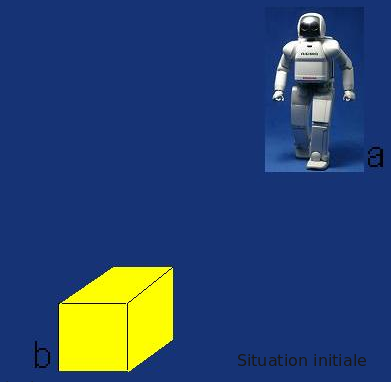
\includegraphics[scale=0.35]{init_tp1.ps} 
     \end{center}
   \end{minipage} \hfill
   \begin{minipage}[c]{.46\linewidth}
     \begin{center}   
      \caption{etat final}
      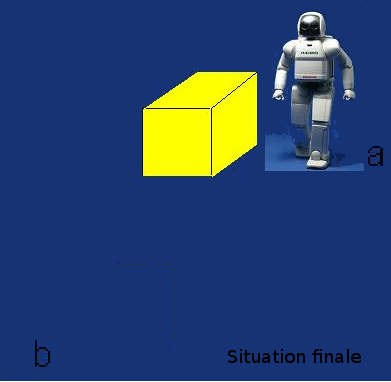
\includegraphics[scale=0.35]{but_tp1.ps}
     \end{center}
   \end{minipage}
   \end{figure}

   Les r\'{e}sultats du test propos\'{e} par le sujet et illustr\'{e} par les images ci-dessus sont donn\'{e} ci-dessous.
   \begin{lstlisting}
   ?- planifier(P5, Temps).

   Profondeur limite : 5.

   P5 = [aller(robot, a, b), prendre(robot, boite), aller(robot, b, a), 
   poser(robot, boite), aller(robot, a, b)] .
   
   Temps = 0.03 s
   \end{lstlisting}

   On pr\'{e}cise que pour n<5, aucun plan n'est trouvé et pour n>=5, on trouve P5.
   
  \subsection{TP2 : planification multi-agents}
 L'objectif ici \'{e}tait de faire de la planification comme au TP1 à la seule différence qu'il y a ici plusieurs agents différents.
 Ce qui offre un nombre de situations plus \'{e}lev\'{e} et des cas plus complexes \`{a} traiter.
 
   \subsubsection{R\'{e}solution du probl\`{e}me}
   La diff\'{e}rence principale avec le TP1 r\'{e}side dans la d\'{e}finition des actions. On a plusieurs agents qui ont des capacit\'{e}s diff\'{e}rentes, il faudra donc
   sp\'{e}cifier les agents capables d'effectuer telle ou telle autre action. De plus, concernant les lieux, un objet peut se retrouver dans la 'main' de tel ou tel autre agent,
   il faut donc un moyen de distinguer les 'mains'. Les objets peuvent aussi \^{e}tre empil\'{e}s les uns sur les autres. La d\'{e}finition des action est donc un peu plus complexe
   comme nous allons le voir dans ce qui suit.
   
   La premi\`{e}re action d\'{e}finie est $aller\_a\_vide(R,Ld,La)$. C'est la possibilit\'{e} pour un agent de se d\'{e}placer de la position Ld vers la position La sans 
   transporter d'objet, ce qui constitue la seule diff\'{e}rence avec l'action aller du TP1. Seul le robot1 sait le faire.
   
   \begin{lstlisting}
   action( aller_a_vide(R,Ld,La),
	[position(R) = Ld, libre(main(R))],
	[position(R) = Ld],
	[position(R) = La] ) :-
	member(Ld,[a,b,c]), member(La,[a,b,c]), member(R,[robo1]), Ld \= La.
   \end{lstlisting}
   
   Ensuite il fallait d\'{e}finir $transporter(R,Ld,La,O)$ qui permet \`{a} un agent R d'aller de la position Ld \`{a} la position La en transportant l'objet O.
   Il faut donc que l'agent et l'objet soient en Ld et qu'il tienne l'objet O. Apr\`{e}s, ils se retrouvent tout les deux en La. Le code est donn\'{e} dans l'encadré ci-dessous.
   
   \begin{lstlisting}
   action( transporter(R,Ld,La,O),
	[position(R) = Ld, position(O) = Ld, lieu(O) = main(R)],
	[position(R) = Ld, position(O) = Ld],
	[position(R) = La, position(O) = La] ) :-
	member(Ld,[a,b,c]), member(La,[a,b,c]), member(R,[robo1]), 
	member(O,[cube1,cube2]), Ld \= La.
   \end{lstlisting}
   
   L'action $attraper(R,O,L)$ d\'{e}crit le fait, pour un agent R, de prendre un objetO sur la table de la position L. Il faut que l'objet soit accessible, c'est \`{a} dire qu'il n'y ait pas d'objet au dessus,
   l'objet n'est donc plus sur la table, n'est plus accessible et la main du robot n'est plus libre. L'objet se trouve maintenant dans la main du robot R.
   Elle peut \^{e}tre ex\'{e}cut\'{e}e par les trois robots.
   
   \begin{lstlisting}
   action( attraper(R,O,L),
	[position(R) = L, position(O) = L, sur(O,table(L)), 
	accessible(O), libre(main(R))],
	[sur(O,table(L)), accessible(O), libre(main(R))],
	[lieu(O) = main(R)] ) :-
	member(L,[a,b,c]), member(R,[robo1, robo2, robo3]), member(O,[cube1,cube2]).
   \end{lstlisting}
   
   L'action $saisir(R,O,L)$ permet \`{a} un robot R de prendre un objet O qui se trouve en haut d'une pile et au m\^{e}me lieu L que le robot.
   La main du robot doit être libre et l'objet doit se trouver sur un autre Osous. Bien s\^{u}, apr\`{e}s l'action, O ne se trouve plus sur Osous,
   il n'est plus accessible et la main du robot n'est plus libre. O est maintenant dans la main de R, et l'objet qui \'{e}tait en dessous est d\'{e}sormais accessible.
   Seuls les robots 2 et 3 peuvent le faire.
   
   \begin{lstlisting}
   action( saisir(R,O,L),
	[position(R) = L, position(O) = L, sur(O,Osous), 
	accessible(O), libre(main(R))],
	[sur(O,Osous), accessible(O), libre(main(R))],
	[lieu(O) = main(R), accessible(Osous)] ) :-
	member(L,[a,b,c]), member(R,[robo2, robo3]), 
	member(O,[cube1,cube2]), member(Osous,[cube1,cube2]), O \= Osous.
   \end{lstlisting}
   
   Les actions $deposer(R,O,L)$ et $empiler(R,Osur,Osous,L)$ sont les actions contraires respectivement à $attraper(R,O,L)$ et $saisir(R,O,L)$, 
   on ne détaillera pas leur fonctionnement. Il suffit de d\'{e}rouler les sc\'{e}narios dans le sens oppos\'{e} \`{a} ceux d'attraper et saisir.
   
   \begin{lstlisting}
   action( deposer(R,O,L),
	[position(R) = L, position(O) = L, lieu(O) = main(R)],
	[lieu(O) = main(R)],
	[sur(O,table(L)), accessible(O), libre(main(R))] ) :-
	member(L,[a,b,c]), member(R,[robo1, robo2, robo3]),member(O,[cube1,cube2]).
   \end{lstlisting}
   
   \begin{lstlisting}
   action( empiler(R,Osur,Osous,L),
	[position(R) = L, position(Osur) = L, lieu(Osur) = main(R), accessible(Osous)],
	[lieu(Osur) = main(R), accessible(Osous)],
	[sur(Osur,Osous), accessible(Osur), libre(main(R))] ) :-
	member(L,[a,b,c]), member(R,[robo2, robo3]), 
	member(Osur,[cube1,cube2]), member(Osous,[cube1,cube2]), Osur \= Osous.
   \end{lstlisting}
   
   \subsubsection{Tests}
   
   Un premier test demandait \`{a} un robot d'inverser deux objets emplil\'{e}s sur une table. Le code est donn\'{e} ci-dessous :
   
   \begin{lstlisting}
   %situation initiale
   initInv(EI) :- EI = [position(robo2) = b, 
		position(cube1) = b, position(cube2) = b, 
		accessible(cube1), 
		libre(main(robo2)), 
		sur(cube1,cube2), sur(cube2,table(b))].
   %situation finale
   butInv(BUT) :- BUT = [position(robo2) = b, 
		position(cube1) = b, position(cube2) = b, 
		accessible(cube2), 
		libre(main(robo2)),
		sur(cube2,cube1), sur(cube1,table(b))].
   \end{lstlisting}
   
   Le r\'{e}sultat de ce premier test.
   
   Un autre test simple consistait \`{a} faire collaborer des robots aux capacit\'{e}s diff\'{e}rentes. Le cube 1 est empil\'{e} sur le cube 2
   en b et il faut les poser en c. Le code est donn\'{e} ci-dessous.
   
   \begin{lstlisting}
   init2Dep(EI) :- EI = [position(robo1) = b, position(robo2) = b,
		position(cube1) = b, position(cube2) = b, 
		accessible(cube1), 
		libre(main(robo2)), libre(main(robo1)),
		sur(cube1,cube2), sur(cube2,table(b))].
   but2Dep(BUT) :- BUT = [position(robo2) = b, position(robo1) = c,
		position(cube1) = c, position(cube2) = c, 
		accessible(cube2), accessible(cube1),
		libre(main(robo2)), libre(main(robo1)),
		sur(cube1,table(c)), sur(cube2,table(c))].
   \end{lstlisting}
   
   Le resultat du deuxi\`{e}me test.
   
   \begin{lstlisting}
   ?- planifier2Dep(P,T).

   Profondeur limite : 9.

   P = [saisir(robo2, cube1, b), attraper(robo1, cube2, b), 
   transporter(robo1, b, c, cube2), deposer(robo2, cube1, b), 
   deposer(robo1, cube2, c), aller_a_vide(robo1, c, b), 
   attraper(robo1, cube1, b), transporter(robo1, b, c, cube1), 
   deposer(..., ..., ...)],
   T = 149.2 
   \end{lstlisting}
   
   Les images ci-dessous illustrent le test du sujet.
   
   \begin{figure}[h]
   \begin{minipage}[c]{.46\linewidth}
     \begin{center}
      \caption{etat initial}
      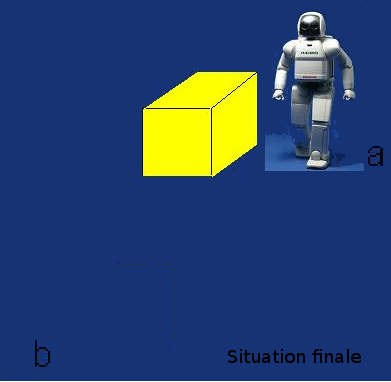
\includegraphics[scale=0.3]{init_tp2.ps} 
     \end{center}
   \end{minipage} \hfill
   \begin{minipage}[c]{.46\linewidth}
     \begin{center}   
      \caption{etat final}
      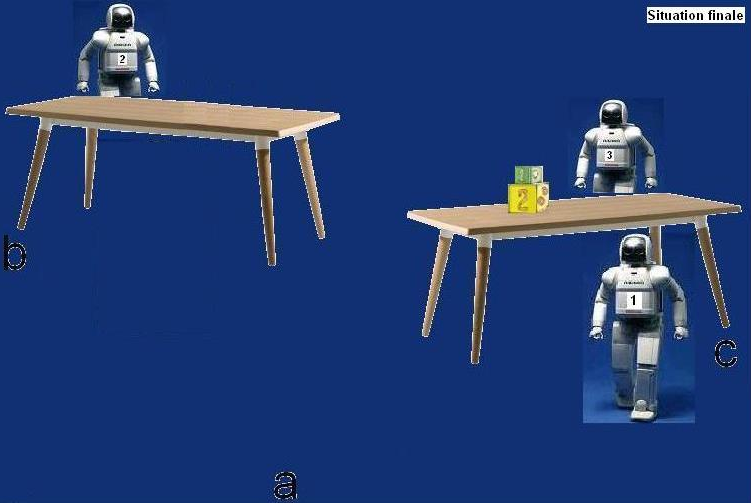
\includegraphics[scale=0.3]{but-tp2.ps}
     \end{center}
   \end{minipage}
   \end{figure}

   Les r\'{e}sultats du test propos\'{e} par le sujet et illustr\'{e} par les images ci-dessus sont donn\'{e} ci-dessous.
   
   \begin{lstlisting}
   ?- planifier(P,T).

   Profondeur limite : 11.

   P = [saisir(robo2, cube1, b), attraper(robo1, cube2, b), 
   transporter(robo1, b, c, cube2), deposer(robo2, cube1, b), 
   deposer(robo1, cube2, c), aller_a_vide(robo1, c, b), 
   attraper(robo1, cube1, b), transporter(robo1, b, c, cube1), 
   deposer(..., ..., ...)|...],
   T = 1055.22,
   \end{lstlisting}
   
  \subsection{TP3 : g\'{e}n\'{e}rateur-d\'{e}monstrateur en logique modale}
  Au cours de cette s\'{e}ance, il fallait \'{e}crire un programme capable de d\'{e}montrer des th\'{e}or\`{e}mes sur une logique modale.
  
   \subsubsection{R\'{e}solution du probl\`{e}me}
   Dans un premier temps il fallait d\'{e}finir le fait qu'une proposition \'{e}l\'{e}mentaire P soit satisfaite dans un monde W. D\'{e}j\`{a}, il faut que P soit bien dans 
   la liste des propositions et W dans la liste des mondes, il suffit que P soit une proposition \'{e}l\'{e}mentaire du monde en question,
   la liste \'{e}tant donn\'{e}e . Cela se d\'{e}finit comme suit :
   
   \begin{lstlisting}
   satisfait(W, P) :-
     proposition(P),
     monde(W),
     m(W,L),
     member(P,L).
   \end{lstlisting}
   
   Mais on ne va pas se limiter \`{a} des formules \'{e}l\'{e}mentaire qui ne contiennent que les propositions list\'{e}es. On veut pouvoir utiliser des op\'{e}rateurs.
   Pour cela il faut d'abord les d\'{e}finir avant de d\'{e}finir l'op\'{e}ration correspondante.
   \begin{description}
    \item[la n\'{e}gation (non) :] c'est un op\'{e}rateur de la forme fy auquel on donnera une priorit\'{e} de 200. Pour que 'non P' soit satisfait dans W,
    il faut que W ne fasse pas parti des mondes dans lesquels P est satisfait. Il faut donc d\'{e}terminer la liste des mondes dans lesquels P est satisfait.
    
       \begin{lstlisting}
   %operateur
   :- op(200, fy, non).
   satisfait(W,non P) :-
     monde(W),
     list_w_satisfait(P, LW), 
     not(member(W, LW)).
   %liste des mondes qui satisfont P
   list_w_satisfait(P, LW) :-
     findall(W,satisfait(W, P), LW).
       \end{lstlisting}
       
    \item[la conjonction (et) :] c'est un op\'{e}rateur de la forme xfy auquel on donnera une priorit\'{e} de 400. Pour que 'P et Q' soit satisfait dans W,
    il faut que P soit satisfait dans W et que Q soit satisfait dans W.
    
       \begin{lstlisting}
   %operateur
   :- op(400, xfy, et).
   satisfait(W, P et Q) :-
     monde(W),
     satisfait(W,P),
     satisfait(W,Q).
       \end{lstlisting}
       
    \item[la disjonction (ou) :] c'est un op\'{e}rateur de la forme xfy auquel on donnera une priorit\'{e} de 400. On utilise ici l'\'{e}criture du 'ou'
    en fonction du 'et et du 'non', en effet 'P ou Q = non(non P et non Q).
    
       \begin{lstlisting}
   %operateur
   :- op(400, xfy, ou).
   satisfait(W,P ou Q) :-
     satisfait(W, non(non P et non Q)).
       \end{lstlisting}
       
    \item[l'implication (=>) :] c'est un op\'{e}rateur de la forme xfy auquel on donnera une priorit\'{e} de 300. L'implication se d\'{e}fini par 'non P ou Q'.
    
       \begin{lstlisting}
   %operateur
   :- op(300, xfy, =>).
   satisfait(W, P => Q) :-
     satisfait(W, non (P et non Q)).
       \end{lstlisting}
       
    \item[l'\'{e}quivalence (<=>) :] c'est un op\'{e}rateur de la forme xfy auquel on donnera une priorit\'{e} de 300. L'\'{e}quivalence n'est rien d'autre qu'une implication dans
    les deux sens.
    
       \begin{lstlisting}
   %operateur
   :- op(300, xfy, <=>).
   satisfait(W, P <=> Q) :-
     satisfait(W, P => Q),
     satisfait(W, Q => P).
       \end{lstlisting}
       
    \item[l'implication stricte (-->>) :] c'est un op\'{e}rateur de la forme xfy auquel on donnera une priorit\'{e} de 300. On a une \'{e}quivalence entre
    'P \-\->> Q' et '\#(P=>Q)', on aura la d\'{e}finition de '\#' un peu plus loin.
    
       \begin{lstlisting}
   %operateur
   :- op(300, xfy, -->>).
   satisfait(W, P -->> Q) :-
     satisfait(W, #(P => Q)).
       \end{lstlisting}
       
    \item[la possibilit\'{e} (<>) :] c'est un op\'{e}rateur de la forme fy auquel on donnera une priorit\'{e} de 200. On dit que P est possible dans W s'il existe
    un monde W2 en relation avec W tel que W2 satisfait P. Il faut donc trouver tous les mondes en relation avec W et voir si il y en a au moins un qui satisfait P
       
       \begin{lstlisting}
   %operateur
   :- op(200, fy, <>).
   satisfait(W, <> P) :-
     monde(W),
     un_rel_satisfait(W,P).
   %une des relations de W satisfait P
   un_rel_satisfait(W, P) :-
     bagof(M, rel(W,M), LM),
     un_satisfait(LM, P).
   %un des éléments de la liste satisfait p
   un_satisfait([M | LM], P) :-
     (satisfait(M,P) -> true; un_satisfait(LM, P)).
       \end{lstlisting}
       
    \item[la n\'{e}cessarit\'{e} (\#) :] c'est un op\'{e}rateur de la forme fy auquel on donnera une priorit\'{e} de 200. Il se d\'{e}finit ais\'{e}ment \`{a} partir
    de la possibilit\'{e}. En effet '\#P = non(<>(non P))'.
    
       \begin{lstlisting}
   %operateur
   :- op(200, fy, #).
   satisfait(W, # P) :-
     satisfait(W,non(<>(non P))).
       \end{lstlisting}
   \end{description}
   
   On rappelle que le but est d'\'{e}crire un programme capable de nous lister toutes les formules d'une certaine complexit\'{e} qui sont des th\'{e}oremes ou de nous
   dire si une formule donn\'{e}e est un th\'{e}or\`{e}me.
   
   Pour cela, on veut d\'{e}j\`{a} \^{e}tre capable de g\'{e}n\'{e}rer toutes les formules d'une certaine complexit\'{e}. Une formule de complexit\'{e} 0 n'est qu'un
   proposition et les formules de complexit\'{e} n sont d\'{e}finies r\'{e}cursivement comme une proposition suivie d'un op\'{e}rateur binaire et d'une formule de
   complexit\'{e} n-1 ou juste comme un op\'{e}rateur unaire suivi d'une formule de complexit\'{e} n-1. Le code est donn\'{e} ci-dessous.
   
   \begin{lstlisting}
   %generation de formules
    genere(P,0):-
      proposition(P).

    genere(F,M):-
      M > 0,
      N is M-1,
      genere(FBIS,N),
      operateur(O),
      proposition(X),
      (O=(=>) -> F=..[O,X,FBIS],F = X=>FBIS;
	O=(<=>) -> F=..[O,X,FBIS],F = X<=>FBIS;
	  O=(et) -> F=..[O,X,FBIS], F = X et FBIS;
	    O=(ou) -> F=..[O,X,FBIS],F = X ou FBIS;
	      O=(-->>) -> F=..[O,X,FBIS],F = X-->>FBIS;
		O=(non) -> F=..[O,X,FBIS],F = non FBIS;
		  O=(<>) -> F=..[O,X,FBIS],F = <> FBIS;
		    O=(#) -> F=..[O,X,FBIS],F = # FBIS).
   \end{lstlisting}
   
   Enfin, il faut \'{e}crire 'theoreme(P)', si P est une variable, on demande la complexit\'{e} des formules \`{a} g\'{e}n\'{e}rer et on les g\'{e}r\`{e}re
   avant de renvoyer celles qui sont des th\'{e}or\`{e}mes, sinon on v\'{e}rifie juste si P est un th\'{e}oreme. P est un th\'{e}or\`{e}me si il est vrai
   dans tout les mondes existant, pour arriver \`{a} cela, on r\'{e}cup\`{e}re la liste des mondes, celle des mondes dans lesquels P est vrai et on v\'{e}rifie
   qu'ils sont \'{e}gaux.
   
   \begin{lstlisting}
   %THEOREME : p doit être satisfait dans tous les mondes
   theoreme(P) :-
	(nonvar(P) ->theoreme_aux(P);
	nl,
	write(' complexite : '),
	read(C),
	nl,
	genere(P, C),
	theoreme_aux(P)).

   theoreme_aux(P) :-
	list_w_satisfait(P, LW),
	findall(W,monde(W), ALLW),
	egal(LW, ALLW)
   %l'egalite est une double inclusion
   egal(LW, ALLW) :-
	inclusion(LW, ALLW),
	inclusion(ALLW, LW).

   %inclusion(C,E) est l inclusion de C dans E
   inclusion([], _). %la liste vide est toujours incluse
   inclusion([W|LW], L) :- member(W,L), inclusion(LW,L).
   \end{lstlisting}
   
  \subsection{TP4 : g\'{e}n\'{e}rateur de plan en logique modale}
  Concernant le TP4, il fallait implanter un g\'{e}n\'{e}rateur de plan en logique modale.
  Le probl\`{e}me \`{a} r\'{e}soudre \'{e}tant :
  
   \begin{lstlisting}
   ?- est(w0,[p1, ... , pk]), satisfait(<<< Plan >>> (F1 ^ ... ^ Fn), w0).
   \end{lstlisting}
   
  Nous supposons l'ensemble des mondes connus. Il nous faut trois nouveaux operateurs '<<', '>>' et '::'. Ils sont d\'{e}fini ci-apr\`{e}s.
  
   \begin{lstlisting}
   %<< a :: b :: c >> (P et Q)
   :- op(100, fy, <<).
   :- op(150, xfy, <<).
   :- op(100, xfy, ::).
   \end{lstlisting}
   
  Il nous faut donc d\'{e}finir ce que c'est que de satisfaire '<<A>>F' dans le monde W. Ici, soit A est une suite d'actions, soit A est une seule action. Soit X la première action de A
  (si A est une suite) ou A lui-m\^{e}me (si A est une action). Il faut que les conditions de X soient v\'{e}rifi\'{e}es dans le monde de d\'{e}part W $est\_entrepeunable(A, W)$,
  il faut ensuite trouver un monde W2 dans lequel les effets de A sont effectifs $est\_effective(A, W)$. Enfin, si A est une action, il faut que F soit satisfait
  dans W2, sinon si A est une suite d'actions 'X::ABIS', il faut que '<<ABIS>>F soit satisfait dans W2. Le code est donn\'{e} ci-dessous.
  
  \begin{lstlisting}
   satisfait(W, << A >> F) :-
	monde(W),
	rel(W, W2), % \E un monde W2
        operateur_act(O),
        (O=(::) -> A=..[O,X,ABIS], %si on a une suite d'actions
                   A = X::ABIS, 
                   est_entrepenable(X, W),
	           est_effective(X, W2),
                   satisfait(W2, <<ABIS>> F);
         est_entrepenable(A, W), %si A est une action
	 est_effective(A, W2),
	 satisfait(W2, F)). % F est satisfait dans W2
   \end{lstlisting}
   
   Il faut donc d\'{e}finir est\_entrepenable et est\_effective. $est\_entrepeunable(A, W)$ permet de v\'{e}rifier que les conditions de A sont satisfaites dans W,
   pour cela, il faut r\'{e}cup\'{e}rer la liste des conditions, la convertir en conjonction de ses diff\'{e}rents \'{e}l\'{e}ments avant de voir si cette conjonction
   est satisfaite dans W. Pour $est\_effective(A, W)$, c'est le m\^{e}me principe mais on prend la n\'{e}gation de la conjonction des effets.
   
    \begin{lstlisting}
  % les conditions de A sont satisfaites dans W
  est_entrepeunable(A, W) :-
	  monde(W),
	  action(A, Cond, Suppr, Ajout),
	  list2conj(Cond, P),
	  satisfait(W, P).

  % les effets de A sont effectifs dans W
  est_effective(A, W) :-
	  monde(W),
	  action(A, Cond, Suppr, Ajout),
	  list2conj(Suppr, SU),
	  list2conj(Ajout, AJ),
	  satisfait(W, non (SU)),
	  satisfait(W, AJ).

  %transforme une liste en conjonction des éléments de la liste
  list2conj([A], A).
  list2conj([A|LA], A et LC) :-
         list2conj(LA, LC)
   \end{lstlisting}
   
   
 \section{Travaux r\'{e}alis\'{e}s lors du bureau d'\'{e}tude}
 Durant le bureau d'\'{e}tude, nous avons \'{e}t\'{e} amen\'{e}s \`{a} analyser diff\'{e}rentes logiques modales et les comparer \`{a} des logiques modales
 vues en cours.
 
  \subsection{Etude de Lm\{p\} }
  
   \subsubsection{Definition de 'n\'{e}cessaire'}
   La d\'{e}finition de 'necessaire' se fait \`{a} partir de celle de 'possible'.
   \begin{lstlisting}
   [p] = ~<p>~ donc 
	|= [p]X <=> |= ~ (<p>(~X))
		<=> |= ~ (p ou ~X) <=> ~(X => p)
		<=> |= ~p et X
   \end{lstlisting}
   
   \subsubsection{Idempotence de 'necessaire' et 'possible'}
   
   Cela revient \`{a} montrer que  
   \begin{lstlisting}
   <p>^n  =  <p><p>...<p>  = <p> et [p]^n  =  [p][p]...[p]  =  [p]
   \end{lstlisting}
   
   On fait une d\'{e}monstration par r\'{e}currence
   \newpage
   \begin{lstlisting}
	Pour n=1, c'est trivial.
	Supposons la propriete vraie au rang n=k
	\A X \in F, on a
	|= <p>^k+1 X <=> |= <p>(<p>^k X)
		     <=> |= <p>(<p>X)
		     <=> |= p ou (<p>X)
		     <=> |= p ou (p ou X)
		     <=> |= p ou X
		     <=> |= <p>X

	de meme pour [p]
	|= [p]^k+1 X <=> |= [p]([p]^k X)
		     <=> |= [p]([p]X)
		     <=> |= ~p et (<p>X)
		     <=> |= ~p et (~p et X)
		     <=> |= ~p et X
		     <=> |= [p]X
   \end{lstlisting}
   On a bien l'idempotence.


   Montrons aussi que toute séquence de modalités $Modi \in {<p>, [p]}$ préfixant une formule X quelconque, 
   telle que $Mod1 Mod2 ... Modn X$, est une formule équivalente à $Mod1 X$.
   Autrement dit :  $Mod1 Mod2 ... Modn  =  Mod1$   pour toute modalité $Modi \in {<p>, [p]}$.
   
   
   Cela revient a dire que la premiere modalite "absorbe les autres", 
   il faut donc montrer que <p>[p] = <p> et [p]<p> = [p]
   \begin{lstlisting}
	\forall X \in F, on a
	|= <p>[p]X <=> |= <p>(~p et X)
		   <=> |= p ou (~p et X)
		   <=> |= (p ou ~p) et (p ou X)
		   <=> |= Vrai et (p ou X)
		   <=> |= p ou X
		   <=> |= <p>X 
	et
	|= [p]<p>X <=> |= [p](p ou X)
		   <=> |= ~p et (p ou X)
		   <=> |= (~p et p) ou (~p et X)
		   <=> |= Faux ou (~p et X)
		   <=> |= ~p et X
		   <=> |= [p]X
   \end{lstlisting}
   
   Avec les propriétés $<p>^n = <p>$ et $[p]^n = [p]$, Cela montre bien que la première modalité "absorbe" les suivantes pour$ Modi \in {<p>, [p]}$.
   
   \subsubsection{Comparaison \`{a} S5}
   
   \begin{lstlisting}
   S5 = {epsilon, <>, []} Union {~, ~<>, ~[]}
   \end{lstlisting}
   
   On a :
   \begin{lstlisting}
   Sigma5 = {epsilon, <p>, [p]} Union {~, ~<p>, ~[p]},
   \end{lstlisting}
   En effet :
   \begin{lstlisting}
   <p><p> = <p>, [p][p] =[p], <p>[p]=<p>, [p]<p>=[p], 
   ~<p> = [p]~ et finalement ~[p] = <p>~,
   \end{lstlisting}
   
   le reste des compositions étant trivial.
   Il y a donc une certaine ressemblance entre Sigma5 et S5. 
   
   
   Mais Sigma5 est-il équivalent à S5? Pour savoir cela, 
   il suffit de voir si les théorèmes caractéristiques de S5 sont aussi vérifiés dans Sigma5.
   
   Les théorèmes vérifiés par S5 sont :
   \begin{lstlisting}
	$\A P,Q \in F$
	(K): [](P => Q) => ([]P => []Q)
	(T): []P => P
	(4): []P => [][]P
	(B): P => []<>P 
	ou 
	(E): <>P => []<>P
   \end{lstlisting}
   
   Essayons de les vérifier dans Sigma5
   \begin{lstlisting}
	\A P,Q \in F, on a :
	(K): [p](P => Q) => ([p]P => [p]Q)
	 <=> [p](~P ou Q) => ((~p et P) => (~p et Q))
	 <=> (~p et (~P ou Q)) => ((p ou ~P) ou (~p et Q))
	 <=> (p ou (P et ~Q)) ou ((p ou ~P) ou (~p et Q))
	 <=> p ou p ou ~P ou (P et ~Q) ou (~p et Q)
	 <=> p ou (~p et Q) ou ~P ou (P et ~Q)
	 <=> ((p ou ~p) et (p ou Q)) ou ((~P ou P) et (~P et Q))
	 <=> Vrai
   \end{lstlisting}
K est vérifié dans Sigma5.
   \begin{lstlisting}
	(T): [p]P => P 
	<=> (~p et P) => P
	<=> ~(~p et P) ou P
	<=> p ou ~P ou P
 	<=> Vrai
   \end{lstlisting}
T est vérifié dans Sigma5
   \begin{lstlisting}
	(4): [p]P => [p][p]P 
	<=> [p]P => [p]P
	<=> Vrai
   \end{lstlisting}
4 est vérifié dans Sigma5.
   \begin{lstlisting}
	(B): P => [p]<p>P 
	<=> P => [p]P
	<=> ~P ou (~p et P)
	<=> (~P ou ~p) et (~P ou P)
	<=> ~P ou ~p
   \end{lstlisting}
Proposition fausse si p et P sont vrais donc B n'est pas vérifié dans Sigma5.
   \begin{lstlisting}
	(E): <p>P => [p]<p>P
	<=> <p>P => [p]P
	<=> (p ou P) => (~p et P)
	<=> ~(p ou P) ou (~p et P)
	<=> (~p et ~P) ou (~p et P)
   \end{lstlisting}
        Proposition fausse si p est faux donc E n'est pas vérifié dans Sigma5.

Sigma5 vérifie donc KT4 mais pas B ni E.
   
   \subsubsection{Modalit\'{e}s}
      Comme on a montré a la section précédente, S5 et Sigma5 ont le même nombre de modalités, on a 
      \begin{lstlisting}
      S5 = {epsilon, <>, []} Union {~, ~<>, ~[]}
      et 
      Sigma5 = {epsilon, <p>, [p]} Union {~, ~<p>, ~[p]}.
      \end{lstlisting}
On a comme règles:
      \begin{lstlisting}
	\A X \in F
	|= epsilon X ssi |= X
	|= <p>X ssi |= p ou X
	|= [p]X ssi |= ~p et X
	|= ~X ssi |= ~X
	|= ~<p>X ssi |= [p]~X 
		 ssi |= ~p et ~X
	|= ~[p]X ssi |= <p>~X 
		 ssi |= p ou ~X
      \end{lstlisting}
      
  \subsection{Etude de Lm\{E0\}}
  
  On généralise cette approche en étudiant la logique  Lm\{E0\}  dédiée aux formules $<\phi>X et [\phi]X où \phi \in Eo = \{p,~p\}$
  
   \subsubsection{Comparaison \`{a} S4}
   
   Les théorèmes vérifiés par S4 sont :
   \begin{lstlisting}
	\A P,Q \in F
	(K): [](P => Q) => ([]P => []Q)
	(T): []P => P
	(4): []P => [][]P
   \end{lstlisting}
	Essayons de les vérifier dans Sigma4 :
   \begin{lstlisting}
	(K): \A P,Q \in F et \A phi \in E0 on a :
	[phi](P => Q) => ([phi]P => [phi]Q) <=> Vrai, 
   \end{lstlisting}
la démonstration se passe comme avec Sigma5. K est vérifié dans Sigma4
De même T et 4 sont vérifiés dans Sigma4.
	
   \subsubsection{Modalit\'{e}s}
   
   On a :

        S4 = { espilon, [], <>, []<>, <>[], []<>[], <>[]<>} Union { ~, ~[], ~<>, ~[]<>, ~<>[], ~[]<>[], ~<>[]<>}

Sigma4 a aussi 14 modalités distinctes :
	\begin{lstlisting}
	Sigma4 = { espilon, <~p>, <p>, [~p], [p], <p>[~p], <~p>[p] } 
	       Union { ~, ~<~p>, ~<p>, ~[~p], ~[p], ~<p>[~p], ~<~p>[p] }
	\end{lstlisting}
On a comme règles:
	\begin{lstlisting}
	\A X \in F
	|= epsilon X ssi |= X
	|= <p>X ssi |= p ou X
	|= <~p>X ssi |= ~p ou X
	|= [p]X ssi |= ~p et X
	|= [~p]X ssi |= p et X
	|= ~X ssi |= ~X
	|= ~<p>X ssi |= ~p et ~X
	|= ~<~p>X ssi |= p et ~X
	|= ~[p]X ssi |= p ou ~X
	|= ~[~p]X ssi |= ~p ou ~X
	|= <p>[~p]X ssi |= p ou (p et X)
	|= ~<p>[~p]X ssi |= ~p et (~p ou ~X)
	|= <~p>[p]X ssi |= ~p ou (~p et X)
	|= ~<~p>[p]X ssi |= p et (p ou ~X)
	\end{lstlisting}

On a de plus les propriétés suivantes :
	
Propriété 1:
	\begin{lstlisting}
	\A X,
	(<p><~p>)X |= p ou ~p ou X |= Vrai ou X |= X 
	donc (<p><~p>) == (<~p><p>) == espilon
	Plus generalement,
	Pour toute modalite Mod, 
	\A n >= 0, (<p><~p>)Mod== (<~p><p>)Mod == Mod
\end{lstlisting}
Propriété 2:
	\begin{lstlisting}
	\A X
	[p][~p]X |= ~p et (p et X) |= Faux et X |= Faux	
	Plus generalement,
	Pour toute modalite Mod, 
	\A X
	([p][~p])(Mod X) == ([~p][p])(Mod X) |= Faux 
\end{lstlisting}
D'où, 
Propriété 2-a:
	\begin{lstlisting}
	<p>[p][~p] X |=  p ou [p][~p]X |= p ou Faux |= p
	\end{lstlisting}
	Propriété 2-b:
	\begin{lstlisting}
	~<p>[p][~p] X |=  ~p  
	avec ~<p>[p][~p] == <~p>[p][~p]
\end{lstlisting}
On vérifie que toute autre combinaison de 3 revient à une modalité précitée.
  
  \subsection{Etude d'autres logiques}
  
   \subsubsection{Lm\{E1\}, E1 = \{Faux\}}
   
	\underline{Modalités :}
	
Lm\{E1\} correspond à Sigma5 avec p = Faux d'où

Lm\{E1\} = \{epsilon, <Faux>, [Faux]\} Union \{~, ~<Faux>, ~[Faux]\}.

avec <Faux> == [Faux] == espilon car

	|= <Faux>X ssi |= Faux ou X |= X

	|= [Faux]X ssi |= Vrai et X |= X
	
Ainsi
\begin{lstlisting}
	 Lm{E1} = {epsilon, ~} soit 2 modalites distintes definies par 
	\A X \in F
	|= epsilon X ssi |= X
	|= ~X ssi |= ~X
\end{lstlisting}
	
	\underline{Propriétés caractéristiques :}
	
Lm{E1} vérifie donc KT4 tout comme Sigma5

De plus,

	(B): P => [p]<p>P 
	
	<=> ~P ou ~p
	
	<=> ~P ou Vrai (dans E1 car p = Faux)
	
	<=> Vrai
	
	Lm{E1} vérifie donc B

	(E): <p>P => [p]<p>P
	
	<=> (~p et ~P) ou (~p et P)
	
	<=> (Vrai et ~P) ou (Vrai et P)   (dans E1 car p = Faux)
	
        <=> ~P ou P
        
	<=> Vrai
	
	Lm{E1} verifie donc E
	
\begin{lstlisting}
	Lm{E1} verifie donc KT4BE comme S5
\end{lstlisting}

   \subsubsection{Lm\{E2\}, E2 = \{Vrai\}}
     
	\underline{Modalités :}
	
Lm{E2} correspond à Sigma5 avec p = Vrai d'où

Lm{E2} = {epsilon, <Vrai>, [Vrai]} Union {~, ~<Vrai>, ~[Vrai]}
	
Ainsi
\begin{lstlisting}
	Lm{E2} = {epsilon, <Vrai>} Union {~, ~<Vrai>} soit 4 
	modalités distinctes definies par 
	\A X \in F
	|= epsilon X ssi |= X
	|= ~X ssi |= ~X
	|= <Vrai>X ssi |= Vrai ou X |= Vrai
	|= ~<Vrai>X ssi |= Faux et ~X |= Faux
\end{lstlisting}
	
	\underline{Propriétés caractéristiques :}
	
Lm{E2} vérifie donc KT4 tout comme Sigma5. De plus,
	
	(B): P => [p]<p>P 
	
	<=> ~P ou ~p
	
	<=> ~P ou Faux (dans E2 car p = Vrai)
	
	<=> ~P
	
	Pas nécessairement vrai donc Lm{E2} ne vérifie pas B

	(E): <p>P => [p]<p>P
	
	<=> (~p et ~P) ou (~p et P)
	
	<=> (Faux et ~P) ou (Faux et P)   (dans E1 car p = Faux)
	
        <=> Faux
        
	Lm{E2} ne verifie donc pas E
	
\begin{lstlisting}
	Lm{E2} vérifie KT4 comme Sigma5
\end{lstlisting}
   
   \subsubsection{Lm\{E3\}, E3 = \{Vrai,Faux\}}
     
Lm{E3} correspond à Sigma4 avec p=Vrai d'où

	Lm{E3} = { espilon, <Faux>, <Vrai>, [Faux], [Vrai], <Vrai>[Faux], <Faux>[Vrai] } 
	
	Union { ~, ~<Faux>, ~<Vrai>, ~[Faux], ~[Vrai], <Vrai>[Faux], <Faux>[Vrai] }
	
	or <Faux> == [Faux] == espilon d'où,
	\begin{lstlisting}
	Lm{E3} = { espilon, <Vrai>,  [Vrai]} Union { ~, ~<Vrai>, ~[Vrai] = Lm{E2}
	\end{lstlisting}
	
	
   \subsubsection{Lm\{E4\}, E4 = \{Vrai,p\} et Lm\{E6\}, E6 = \{Vrai,Faux,p\}}
     
   On sait que <Faux> == [Faux] == espilon
	donc 
	\begin{lstlisting}
	Lm{E4} == Sigma4, Lm{E6} = Lm{E5}.
        \end{lstlisting}
        
        
   \subsubsection{Lm\{E5\}, E5 = \{Faux,p\}}
     
	
	Pour toute modalité Mod, on a,
	
	|= <Vrai>ModX ssi |= Vrai 

	|= ~<Vrai>ModX ssi |= Faux

	|= Mod<Vrai>X ssi |= Mod(Vrai)

	|= Mod~<Vrai>X ssi |= Mod(Faux)
	
	et [Vrai] == ~<Vrai> et ~[Vrai] == <Vrai>
	
	Ainsi Lm{E5} se réduit à Lm{E2} Union Sigma5, soit
	\begin{lstlisting}
	Lm{E5} =  {epsilon, <Vrai>, <p>, [p]} Union {~, ~<Vrai>, ~<p>, ~[p]}
        \end{lstlisting}
	
	
	
   \subsubsection{Lm\{E7\}, E7 = \{Vrai,Faux,p, ~p\}}
   
     \begin{lstlisting}
    %<Faux> et [Faux] sont neutres donc
    Lm{E7} = Lm{Vrai, p, ~p}
	   = Lm{E2} Union Sigma4  %par le meme raisonnement que precedemment
	\end{lstlisting}
   
   \subsubsection{Lm\{E8\}, E8 = \{p,q\}}
    
        ( Lm\{p\} $\cup$ Lm\{q\} ) est inclus dans Lm{E8}.

	On a :
	
	<p><q> == <q><p> et est idempotent (car le 'ou' est commutatif et 'X ou X == X')
	
	[p][q] == [q][p] et est idempotent (car le 'et' est commutatif et '~X et ~X == X')
	
	avec :
	
	|= <p><q>X ssi |= p ou q ou X

	|= [p][q]X ssi |= ~p et ~q et X

	|= ~<p><q>X ssi |= ~p et ~q et ~X

	|= ~[p][q]X ssi |= p ou q ou ~X

	
	p et q jouent des rôles symétriques.
	
	|= <p>[q]X ssi |= p ou (~q et X) |= (p ou ~q) et (p ou X)

	|= ~<p>[q]X ssi |= ~p et (q ou ~X) |= (~p et q) ou (~p et ~X)

	|= [p]<q>X ssi |= ~p et (q ou ~X) |= (~p et q) ou (~p et ~X)  donc [p]<q> == ~<p>[q]
  
 \section{Conclusion}
      Ce projet nous a permis de nous familiariser avec avec la programmation en Prolog et de nous rendre compte de la puissance de ce language et des possibilités presque 
      infinies qu'il offre. Il nous a aussi permis d'avoir une meilleure compréhension de la notion de planification et de la manipulation des logiques modales. Nous avons
      été agréablement surpris de la complexité des résultats que l'on peu obtenir avec très peu de code.
 
 
  
\end{document}